% End-to-end inference time for one full multi-field cone (x_HI + T_b).
% Numbers: CompAstro wiki, "Rhizome Neural Operator Results" §7.
\documentclass[border=4pt]{standalone}
\usepackage[T1]{fontenc}
\IfFileExists{fourier.sty}{\usepackage{fourier}}{\usepackage{lmodern}}
\usepackage{amsmath}
\usepackage[dvipsnames]{xcolor}
\usepackage{pgfplots}
\pgfplotsset{compat=1.16}
\begin{document}
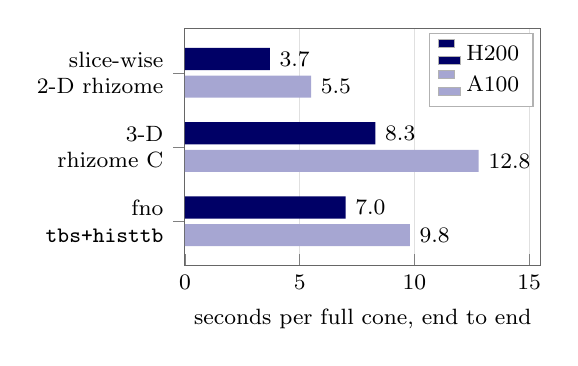
\begin{tikzpicture}
\begin{axis}[
    xbar, bar width=8pt,
    width=6.1cm, height=4.6cm,
    xmin=0, xmax=15.5,
    xlabel={seconds per full cone, end to end},
    xlabel style={font=\footnotesize},
    symbolic y coords={fno,rh3d,rh2d},
    ytick=data,
    yticklabels={{fno\\\texttt{tbs+histtb}},{3-D\\rhizome C},{slice-wise\\2-D rhizome}},
    yticklabel style={font=\footnotesize, align=right},
    tick label style={font=\footnotesize},
    enlarge y limits=0.3,
    xmajorgrids, grid style={black!12},
    nodes near coords, nodes near coords style={font=\footnotesize, anchor=west}, point meta=explicit symbolic,
    legend style={font=\footnotesize, at={(0.98,0.98)}, anchor=north east, draw=black!30},
    legend cell align=left, reverse legend,
    axis line style={black!60},
    ytick pos=left, xtick pos=bottom,
  ]
  \addplot[fill=NavyBlue!35, draw=none] coordinates {(9.8,fno) [9.8] (12.8,rh3d) [12.8] (5.5,rh2d) [5.5]};
  \addplot[fill=NavyBlue!80!black, draw=none] coordinates {(7.0,fno) [7.0] (8.3,rh3d) [8.3] (3.7,rh2d) [3.7]};
  \legend{A100, H200}
\end{axis}
\end{tikzpicture}
\end{document}
